% Standalone section for the ICLR manuscript.
% Requires graphicx. Include scaling_ablation_appendix.tex in the appendix.
% These are downstream NWM results, not standalone LAM reconstruction results.
\section{Scaling and Ablation Studies}
\label{sec:scaling_ablation}

We examine how the amount of unlabeled video used for latent-action
learning affects downstream visual prediction. For this ablation, we
compare four latent-action pretraining settings that retain 25\%, 50\%,
75\%, or 100\% of the unlabeled data pool. We denote this percentage by
$U$ and keep the action-label availability percentage fixed at $L=100\%$.
Each resulting model is then fine-tuned with real actions using the same
downstream architecture, hyperparameters, and fine-tuning schedule.
We evaluate all four models on the same 500 RECON windows for direct
4\,s prediction, with ground-truth action conditioning, EMA weights,
and 250-step DDPM sampling. We report the mean DreamSim over these
predictions; lower values indicate greater perceptual similarity to
the ground-truth images.

\begin{figure}[t]
  \centering
  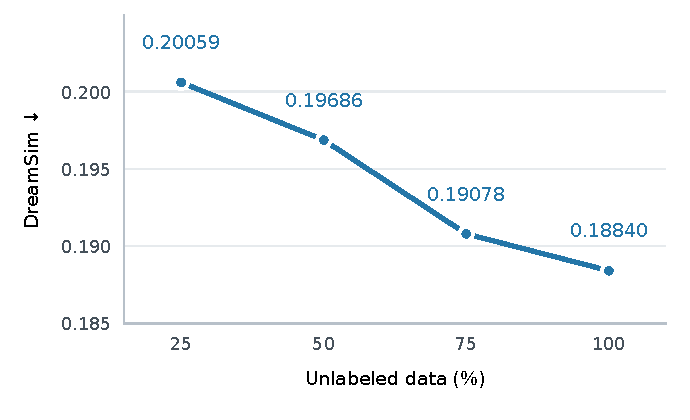
\includegraphics[width=0.68\linewidth]{figures/data_scaling/data_scaling.pdf}
  \caption{\textbf{Scaling unlabeled data on RECON.}
  The horizontal axis gives the percentage of the unlabeled data pool
  used for latent-action pretraining ($U$), with action-label availability
  fixed at $L=100\%$. After the same downstream real-action fine-tuning
  procedure, all four models are evaluated on the same 500 RECON windows
  for direct 4\,s prediction. DreamSim decreases monotonically, with a
  6.08\% relative reduction from 25\% to 100\% data. Lower is better.
  Points are single-checkpoint, single-evaluation-seed estimates;
  lines connect measurements without fitting a scaling law.}
  \label{fig:data_scaling}
\end{figure}


\paragraph{Scaling unlabeled data.}
Figure~\ref{fig:data_scaling} shows a monotonic decrease in RECON
DreamSim: 0.20059, 0.19686, 0.19078, and 0.18840 at $U=25\%$, $50\%$,
$75\%$, and $100\%$, respectively. Using the full unlabeled data pool
reduces DreamSim by 6.08\% relative to the 25\% setting. The improvement
continues from 75\% to 100\%, although this final gain is smaller than
the preceding increment. These observations support the benefit of
scaling unlabeled video for perceptual prediction quality on RECON
under the fixed $L=100\%$ setting. Each point corresponds to one trained
checkpoint and one evaluation seed; the trend is descriptive and does
not establish a universal scaling law. Evaluation details and the four
point estimates are provided in Appendix~\ref{app:data_scaling}.
